%%%%%%%%%%%%%%%%%%%%%%
\documentclass{doublecol-new}
%%%%%%%%%%%%%%%%%%%%%%

\usepackage{natbib}
\usepackage{html}
\usepackage{url}

\usepackage[utf8]{inputenc}
\usepackage{lmodern}

\def\newblock{\hskip .11em plus .33em minus .07em}

\makeatletter
\def\theequation{\arabic{equation}}

\JOURNALNAME{\TEN{\it Int. J. of Systems, Control and
Communications, Vol. \theVOL, No. \theISSUE, \thePUBYEAR}\hfill\thepage}%

\def\BottomCatch{%
\vskip -10pt
\thispagestyle{empty}%
\begin{table}[b]%
\NINE\begin{tabular*}{\textwidth}{@{\extracolsep{\fill}}lcr@{}}%
\\[-12pt]
Copyright \copyright\ 2016 Inderscience Enterprises Ltd. & &%
\end{tabular*}%
\vskip -30pt%
%%\vskip -35pt%
\end{table}%
} \makeatother

%%%%%%%%%%%%%%%%%
\begin{document}%
%%%%%%%%%%%%%%%%%

\setcounter{page}{1}
\LRH{G. L. Camillo and C. M. Westphall}
\RRH{Privacy Preserving in finer grained access control using XACML and OpenID Connect}
\VOL{x}
\ISSUE{x}
\PUBYEAR{xxxx}
\BottomCatch
\CLline
\PUBYEAR{2015}

\subtitle{}

\title{\sf{\textbf{Privacy preserving in finer-grained access control using XACML and OpenID Connect}}}

\authorA{\sf{Gerson Luiz Camillo*,Carla Merkle Westphall}}

\affA{Departamento de Informática e Estatística (UFSC-CTC-INE),\\
	Universidade Federal de Santa Catarina,\\	
	Laboratório de Redes e Gerência,\\	
	CEP 88040-900 - Campus Universitário
	Florianópolis, Santa Catarina, Brasil	
	Phone: +55 048 3721-  \\
E-mail: gerson.camillo@posgrad.ufsc.br\\
E-mail: carlamw@inf.ufsc.br\\
{\sf{*}}Corresponding author}

\begin{abstract}
Many service providers have started implanting personalization in their web portal so that an individual needs not only to submit the assurance of digital identity but also to reveal Personally Identifiable Information (PII), known as attributes in the context of control access. The disclose of PII represents a privacy problem. This paper offers a model that allows for the individual to obtain services without the need to report PII, but only the results of the politics of fine granulation over the value of the attribute. We also present an implementation of a prototype in addition to a case representing a hypothetical scenery for evaluation. The project demonstrated that for certain situations an user can restrict the publication of certain PII and still gain access to services.

Brings the fine-grained authorization to the world of open and lightweight identity management through the use of XACML 3.0 and OpenID Connet.  
\end{abstract}

\KEYWORD{access control; XACML; federated identity management; OpenID Connect; privacy preserving.}

\REF{to this paper should be made as follows: Camillo, G.L. and Westphall, C.M.. (2015) `Privacy preserving in finer-grained access control using XACML and OpenID Connect', {\it Int. J. Security and Networks}, Vol.~x, No.~x, pp.xxx--xxx.}

\begin{bio}
Gerson Luiz Camillo received his BSc in Computer Science from the Universidade Federal de Santa Maria, RS, Brasil. His research interests include security, access control and identity management.\vs{8}

\noindent Carla Merkle Westphall is a Professor in the Departamento de Informática e Estatística of Universidade Federal de Santa Catarina (UFSC) Brazil. She is working in security since 1996. Her research interests include information security, distributed security, identity management and cloud security. She received her PhD in Electrical Engineering (Information Systems Security) from the Universidade Federal de Santa Catarina. She is a member of the Networks and Management Laboratory which has many master and doctoral students developing security research.

\end{bio}

\maketitle

\section{Introduction}

The technologies of authentication and authorization have been evolving in matters of security, usability, and performance in order to accommodate to the context of service distribution in the web. The browser became the main interface to the utilization and diffusion of information, as well as to the access to online resources. The data that identifies and distinguishes the user have acquired inestimable value in the digital society, to the extent that any transaction online usually requires that some information is disclosed. This data is represented by attributes and is known as Personally Identifiable Information (PII). The relationship between the traces we leave while navigating on the Internet and the information that identifies us has allowed the development and rising of Internet giants such as Google and Yahoo.

MOTIVAÇÃO: por que é importante PRIVACIDADE.
The privacy aims to control and protect both data owns by a user and the PII proving law, techniques and mechanisms to empower the entity about its information. Specificaly, in the area of computer security, privacy is about minimizing the personal information released and/or prevent that attributes has been linked to the user \citep{gurses2011engineering,heurix2015taxonomy,landwehr2012privacy}. Privacy was subject a concern a long time ago. The importance of protect personal data levou às primeiras iniciativas de regulação. And the first normative was established in 1981 with guidelines to protect the privacy of personal data in EU \citep{oecd1981guidelines} with the establishment of eight principles. These principles influenced the criation of directives, laws and frameworks around the world. The importance of privacy today is reflected in the revision of the guidelines \citep{oecd2013guidelinesupdated} and the consequences in the form of companies work with personal data \citep{kuschewsky2014new}. 

POR QUE É IMPORTANTE RESOLVER O PROBLEMA: exemplos de aplicações
To understand the driving problem [driving problem of what?] we present the scenario of a library, as used in the paper of \citep{camenisch2014concepts}. The librarian cannot lend titles (books, films) to underage persons. To further the community use, the library will send free of charge books to people who are 60 or older and who live in the central area of the city. Considering the service will include the option of preserving the privacy of user data, how can we create a solution that allows the individuals to use the service without exposing personally identifiable data? This question comprises two sides of service negotiation: the service provider needs to guarantee the restriction on using some services and the user doesn't want to disclose personal information.

O QUE O PRESENTE TRABALHO TEM DE INOVADOR em relação aos outros trabalhos, CONTRIBUIÇÃO:
The above problem prompted the search of related works and systems that presented solutions to achieve privacy in the use of online services. The context of the problem and the proposals of this work parallel service provider (SP) enforcing fine-grained policies [and] personally attributes managed by an identity provider (IdP). Both are executed in disjunct security domains. Specifically, the SP runs XACML and the IdP, OpenID Connect, under Representational State Transfer (REST) services and protocols. The only paper that handled with these devices in the setting of privacy preserving was \citep{ma2015cloud}, but in that case, the policy manager was in the same domain of the identity provider. The Privacy-preserving Attribute-based Credentials (Privacy-ABCs) technologies \cite{camenisch2009credential,dagdee2011extending} offers solutions for privacy-preserving of PII robustness of underlying cryptography, but is a complex system. The User-Managed Access (UMA) profile of OAuth 2.0 \cite{hardjono-oauth-umacore-14} is an alternative to authorization in Web 2.0 that can be integrated with OpenID Connect bringing novel perspectives to user management of control access. But UMA depends strongly on the user defining policies and on the resource server to enforce such policies (there is a step that establishes a trust relationship between the entities). 

We present in this paper a different approach, that permits the user to minimize the personal information released to the service provider resource server while still maintaining access to resources/services. It is not necessary to trust the service provider because it trusts the user possesses the required attribute. The idea has similarities with the Privacy-ABC technologies, but the proposed model is supported by recent protocols and specifications, like OAuth 2.0, OpenID Connect for identity management and RESTful as the means of transportation. Aside, the service provider applies fine-grained authorization using XACML architecture and policies.


The main contributions of this work are: introduction of a framework that evaluates attribute-based access control policies in the identity provider, returning to the service provider only the results of the evaluation, aiming to prevent the service provider from obtaining private user data; the enforcement by the service provider of fine-grained access control policies using XAML while keeping user privacy regarding PII; and the proposal of a prototype to assay a use case scenario.

The remaining of this paper is arranged as follows: Section 2 presents the related works; Section 3 discusses access control, identity, and privacy; in Section 4 the proposal is presented; Section 5 exposes the development; the results are displayed in Sections 6, and 7 has some summing-ups and the description of future works.

\section{Related works}
There is a broad range of solutions to enhancing privacy in systems that supply services using or providing data relative to a person. These systems are known as Privacy Enhancing Technologies (PET). A lot of PET and proposals have the purpose of augmenting or establishing privacy in the relationship between users and service providers when some form of personal data is involved. The range extends itself from Cookie-cutters blocking cookies and language privacy of Platform for Privacy Preferences (P3P) to cryptographic solutions that incorporate third-party authorities, such as the Privacy-Attribute Based Credentials (Privacy-ABC). To restrict the works analysed and compared, we narrow it to the privacy of personal data, as defined in EU Directive 95/46/EC\cite{directive199595}, that refers to the piece of information that identifies directly or indirectly a natural person. As we are working on data minimization, we omitted the proposal that addresses how data is used, according to \citep{mondal2014beyond}.

\citep{kolter2007privacy} was one of the first papers that searched for answers to the question of privacy in systems of attribute-based access control about Service-oriented Architectures (SOA). The author extended the XACML platform to support PDPs detached from the service provider. This architecture allows the users that access the service to define their privacy preferences, which determines the choice of  most adequated PDP. However, it requires that the service provider trusts the decision designed by particular PDP. Trust issues in the transport of authorizations were addressed through public key infrastructure. An important concept introduced was the association of different PDPs to privacy profiles; however, the paper doesn't present a prototype because the model was expected to be included in project Access-eGov\cite{pernulAccesseGov}.


An approach to privacy preserving PII is the authentication based on Attribute-based Credentials that consists of a list of attribute-value pairs certified cryptographically by an issuer. The basic operation on Privacy-ABC credentials are the same as the X-509 certificates. But the realization of the Privacy-ABC is based on different cryptographic primitives, such as pseudonym systems\citep{chaum1981untraceable}, anonymous credentials\citep{camenisch2001efficient}, self-blindable credentials\citep{verheul2001self}, and minimal disclosure tokens\citep{brands2000rethinking}.

Two projects founded in EU worked on identity management using Privacy-ABC technologies. The research project Privacy and Identity Management for Europe (PRIME) is a system for privacy-enhancing identity management that combines anonymous credentials with attribute-based access control, and anonymous communication. \cite{ardagna2008privacy} and \cite{ardagna2010exploiting} presented works related to the project that allow individual prove the possession of condition to satisfy the restrictions imposed by services on attributes without revealing personal information. The concepts of project achieved little practical applications in real world, because areas of user interfaces, policy languages, and infrastructure needed further research \citep{ardagna2010enabling,bichsel2013h2}. Between 2008 and 2011 the work continued in the project Privacy and Identity Management in Europe for Life (PRIMELife) que tinha por objetivo apresentar soluções in identity management, integrating access control policy with privacy-preserving data handling policies. \cite{ardagna2010enabling} apresentou uma solução de controle de acesso baseado também em certificados de atributos mas usando padrões de mercado, no caso XACML \citep{rissanen2013extensible} e SAML \citep{ragouzis2008security}. O primeiro, para autorização baseada em atributos, enquanto o segundo como um meio de transporte de declarações sobre fatos de autenticação e/ou autorização. No artigo o autor somente apresentou o modelo, não incluindo testes de validação de um possível protótipo, considering that the implementation was occurring in PRIMELife project. The projects PRIME and PrimeLife and the related works demonstrated the difficulty to applied the technologies to the production environments \cite{bichsel2013h2}.

The Privacy-ABC has two instantiating technologies that received commercial support. They are the IBM Identity Mixer (IDEMIX)\citep{camenisch2002design} that is based on the scheme proposed by \cite{camenisch2001efficient} and the Microsoft U-Prove, specification defined by \cite{brands2000rethinking}. The core features of those technologies are: pseudonymity, the selective and minimal disclosure of attributes, untraceable of user authentications and unlinkability between of the revealed data by service providers. To use in online services the credential is transformed in a presentation token, that can be verified cryptographically. Another application of Privacy-ABC are electronic credentials based on smart cards exemplified by the project IRMA (I Reveal My Attributes)\citep{koning2014abc}. A project known Attribute-based Credentials for Trust (ABC4Trust) founded by EU has the goal to address the federation and interchangeability of technologies related to Privacy-ABC. The establishment of the project reflects the difficulty of applicability of the technology in real world systems. The drawback of Privacy-ABCs technologies are the relative complexity \citep{nogueira2014aprimoramento} of the infrastructure needed for emission, verification and revocation of tokens and certificates. The slow adoption was caused mainly by the difficulty of use the technology \citep{camenisch2012language}. Another question is the assumption of a central authority \citep{bertino2011identity}. As a technology based on public-key infrastructure the revocation of certificates are a harder problem to be solved. Compared to our proposal, one difference is the approach of privacy issue attacked by the system: we consider the identity provider trustworthy while the Privacy-ABC considerer that online identity provider can't be trusted. Furthermore they not address the RESTful services, fine-grained authorization based on XACML and user attributes given by an identity providers OAuth-based.

\cite{kounga2010extending} também seguiu a linha de estender o XACML, mas definindo uma autoridade que armazenasse os atributos e políticas. A proposta de Kounga em \cite{kounga2010extending} aborda a possibilidade de que o consentimento do usuário pode se estender tanto nas preferências de privacidade das informações pessoais quanto em dados. Além disso, através da extensão do XACML o consentimento pode ser de granularidade mais fina sobre os dados. Para evitar que os pontos PDP e PEP do XACML não tenham acesso às preferências de privacidade e de dados do usuário a arquitetura foi estendida para incluir módulos que tratam exclusivamente dos dados de atributos, que foi definido como \textit{Attribute Authority} (AA). Apesar de apresentar a característica de autorização com privacidade, a solução necessita que uma autoridade de confiança (chamada de \textit{data collector}) gerencie as preferências e os dados pessoais. Além disso, o artigo não apresentou uma implementação da proposta, em parte, devido ao fato da solução usar alguns conceitos e estender o framework do projeto \textit{Identity Governance Framework} (IGF). A extensão do XACML para acomodar controle de acesso baseado em certificados de atributos foi explorada pelos trabalhos de \cite{camenisch2009credential} e \cite{dagdee2011extending}, o primeiro na forma de uma linguagem e outro na extensão da arquitetura.

\cite{chadwick2012privacy} propôs uma arquitetura em  que fornece serviço de autorização para ambiente em cloud. A questão de privacidade é tratada sob dois aspectos: primeiro, através de diferentes PDPs que avaliam cada qual uma linguagem de política de privacidade diferente; e o conceito de \textit{sticky policy}, que permite que os dados trafeguem entre instalações de nuvens mas mantendo presa a política de privacidade. O pressuposto adotado no trabalho foi que os provedores de serviço na nuvem são confiáveis de tal forma que vão honrar as políticas de privacidade definidas nas sticky policies oriundas de outros provedores no mesmo ambiente de nuvem. Trata-se de proposta dentro do projeto PERMIS \cite{chadwick2008permis} that is framework to provide policy based authorisation for federated and/or grid applications using the standard SOAP/SAML protocol. The goal of the project is create a system with privacy preserving authorization and tools for management of policies. The architecture was defined and constructed over the SAML protocol and the entity that provide de user data was not specified by \cite{chadwick2012privacy} but PERMIS can be integrated with Shibboleth and Globus toolkit, while our proposal uses RESTful and OpenID Connect. Although the user has control of his privacy PII, the model depends on the service provider respect the policy.

Architectures for policy decomposition \cite{lin2008policy} and policy federation \cite{decat2012toward,decat2013federated,decat2014middleware} aimed to provide confidentiality and privacy when enforcing access control policies in distributed environment. The proposed works are supported by the XACML policy and architecture, because the entities are specified to be easy distributed. The proposed works are supported by SOAP/SAML protocols and the relationship with identity providers were not defined in their proposals. 

The identity management consolidated the externalization of user authentication. The domain service that maintains the attributes and the identities are outside of the resource domain. An example of well know package for web single sign-on and for identity federation is the open source Shibboleth \citep{erdos2002shibboleth}. It's based on OASIS Security Assertion Markup Language (SAML) and in Shibboleth version 2.0 the OpenSAML is the stack that provides the XML support. For the purposes of this work the Shibboleth don't or partially meets the requisites, because of this considerations: Shibboleth uses SAML and it is a SOAP/XML based protocol; the SAML infrastructure for federation needs explicit trust configuration; and the service providers based on SAML and Shibboleth are tightly coupled to the identity providers. Those characteristics difficult the adoption for a Web more light, based on RESTful Web API and desktop/mobile based. Another recent system for identity management is the OpenID Connect, which is defined as identity layer on OAuth 2.0. The main advantages are the use of RESTful Web APIs and JSON for transport the user assertions. However the two mentioned protocols don't have the aim to provide fine-grained authorization, only the authentication of user and transport of claims about it.

Externalization of authorization in Web applications took to the protocols OAuth and User-Managed Access (UMA)\citep{hardjono-oauth-umacore-14,machulak2010user}. The OAuth 2.0 provides a mechanism to a user authorize third-party applications access his or her resources without expose private credentials. For that online services on behalf of user, the protocol uses access tokens as credentials. The flow of messages is based on JSON and the access through open APIs. The UMA protocol is a profile of OAuth 2.0 in that the user manages the policy of access control to his protected resources (personal data, content or services). This is achieved by the user defining the policies in a central authorization server (AS) and the requesting parties (RP) adhering to a set of obligations \citep{maler-oauth-umatrust-03}. Resuming, UMA is a protocol for authorization in Web 2.0 that leverage to the user of control about his data, that is, the UMA is user-centric while our proposal is centred in service but offering privacy about PII. Another difference is that the UMA needs agreement between authorization server and requesting party that possibilities the AS trust that the RP enforces the user defined policies while ours concept is that the RP is untrusted.

\cite{werner2015approach} presented an approach and in \cite{werner2016model} a model for an identity management with privacy in cloud infrastructure. The model comprises a IdM in cloud where SP and IdP in work together through interactions to permit users consume services in a environment with the next characteristics: user receiving trust information based on reputation and risk analysis of SP, minimization of release of personal attributes, obfuscation of user activities through anonymity and pseudonyms, and the possibility of user defining the privacy policy related to the disclose of data to the cloud. Even though the authors presented a model with attempt to help users in making decision about her or his privacy, the architecture depends on the SP enforce the privacy policy. Concerning the PII, our proposal permits the user access services protected by fine-grained policies and without releasing information about certain attributes.

O trabalho de \cite{ma2015cloud} apresentou um modelo em que os usuários eram identificados por uma federação \textit{OpenID Connect} e o controle de acesso através do XACML. Para incluir o consentimento dos usuários sobre a liberação de seus dados, foi criado um servidor de políticas XACML ligado ao servidor de identidade. O mérito da proposta é a inclusão de um servidor de políticas XACML ligado ao servidor de identidade \textit{OpenID Connect}. Essa solução permitiu descrever os escopos e atributos mais complexos em termos de linguagem de controle de acesso do XACML. Apesar de usar padrões atuais, a solução de Ma foi adaptada especificamente para resolver a questão do acesso de pacientes, médicos e colaboradores sobre os dados de imagens de diagnóstico médico disponibilizados por diferentes clínicas e hospitais dentro de uma nuvem.



\section{Background and Context}
This section discusses the main topics that are related to the context of this work. Specifically, access control, identity management and privacy.

The access control is the centre of security of any information system asset and resides in all levels, from hardware to application \citep{anderson2008security}. The main goal of access control is mediate requests to resources and enforce the decision of grant or deny \citep{samarati2001access}. But, as denoted by \cite{gollmann2011compsecurity}, the process of controlling access is evaluated in two steps: authentication and authorization. The authentication is the mechanisms that verifies with trustworthy the identity of the entity that is requesting access to resources. Authorization is the process of regulating the access control. With the complexity of interactions between consumer and provider of services and the increasing of online services took the outsource of the procedures of authenticate and authorize users and applications. Our work has based on those protocols and systems.

Sistemas de controle de acesso baseados em identidade assumem que a autenticação foi realizada e o principal foi identificado com sucesso. Os três sistemas clássicos de ampla adoção e que são baseados no princípio mencionado são: the Discretionary Access Control (DAC); the Mandatory Access Control (MAC); e o mais recente, the Role Based Access Control (RBAC). O controle de acesso discricionário \cite{lampson1974protection} se baseia em uma matriz de acesso constituída de domínios de proteção (usuários e objetos) cuja principal característica é o fato deste modelo delegar a política de segurança para o usuário, ou seja, as entidades controlam quem e como pode realizar determinado acesso. O modelo que foi proposto a seguir foi o Role-Based Access Control (RBAC), que foi formalizado por \cite{ferraiolo1992role} e cuja principal motivação foi atender ao estabelecimento de políticas de controle de acesso em ambientes corporativos. A característica principal deste modelo é a separação da ligação direta entre os usuários e as respectivas permissões. Aos papeis são associados conjuntos de permissões que regulam as operações sobre os objetos.

A evolução da computação trouxe questões que modelos tradicionais de controle de acesso baseados em identidade já não podiam satisfazer. As mais importantes foram: o usuário já não está mais definido; a computação agora é realizada tanto no servidor quanto no cliente; políticas de controle de acesso evoluíram para considerar aspectos tanto do sujeito quanto do objeto e questões ambientais relativas às operações. Essa e outras necessidades levaram à formalização of model Attribute Based Access Control (ABAC), definido formalmente em \cite{huABAC2014guide}: o controle de acesso aos objetos é obtido pela avaliação de regras considerando os atributos das entidades (sujeito e objeto), das operações e do ambiente, relevantes para a requisição. O modelo conta com várias entidades, que realizam diferente funções, permitindo a implementação distribuídos desses unidades.

The entities that compose the ABAC were first defined in the Recommendation X.812 da ITU-T, de 1995 \citep{itut1996acframework} and each point has specific function. The Policy Decision Point (PDP): avalia a política aplicável à requisição que resulta em uma decisão de autorização, que é retornada para a entidade responsável por cumprir a política. The Policy Enforcement Point (PEP) is the entity efetivamente realiza o controle de acesso, protegendo o recurso. Recebe as requisições de acesso e as envia para o PDP for evaluation and cujas respostas de autorização definem o cumprimento da política. The policy are created and maintained by the Policy Administration Point (PAP). An important entity in the ABAC model is the Policy Information Point (PIP), which serve como repositório e origem para os atributos necessários à avaliação da política.

Ao lado das muitas vantagens, há alguns problemas, dois dos quais serão apresentados pela sua importância: o primeiro é que todos os participantes na autorização ABAC devem concordar com o significado dos atributos \citep{karp2010abac,Rubio-Medrano2015federated} e também há necessidade de definir os atributos relevantes para o controle de acesso; e, em segundo lugar, the Policy Enforcement of Policy devem ser implementados em todos os recursos que deverão ser protegidos pelo ABAC.

The Organization for the Advancement of Structured Information Standards (OASIS) defined the standard eXtensible Access Control Markup Language (XACML)\cite{rissanen2013extensible} based on the advantage of ABAC for fine-grained authorization. The XACML describes the core parts: a policy language express in XML; a request-response protocol and a reference architecture. The decoupled architecture is almost the same as specify in \cite{huABAC2014guide} and \cite{itut1996acframework} but with the inclusion of Context Handler, that mediates the communication between the components.

The language of XACML define the policy that the architecture needs to evaluate and enforce. The top-level policy elements are \textit{PolicySet}, \textit{Policy}, and \textit{Rule}. The PolicySet contains set of PolicySet and set of Policies. The Policy in turn contains one or more Rule elements and as such is the elementary unit of evaluation of the policy by the PDP. The Rule has three main parts: Target which denotes rule’s applicability to the authorization request, Conditions which are authorization predicates over attributes, and Effect is the result of the rule evaluation. It returns either “Permit” or “Deny” if the rule is satisfied and “Non Applicable” if the Target and/or Conditions are not satisfied. The Policy returns "Indeterminate" when the PDP is unable to evaluate the request, by error or by missing attributes. The Target element can be included in all the top-level elements (PolicySet, Policy, and Rule) and it cat be considered as an applicability filter on subject, resource, action and environment attributes. The Target element of Policy index the policies and it permits the PDP to determine the applicable policy for the request. The Obligation and Advice expressions are returned with the decision to the PEP and they inform the actions that the enforcement point need take along with the decision of request. The difference between them is that the Advice element may be safely ignored by PEP. When there are multiples Rule elements with each one resulting in a decision and when there are more than one Policy elements in a PolicySet container, there are a mechanisms that decide the final outcome of Rule/Policy evaluation. For that, the PolicySet defines a \textit{policy combining algorithm} and a \textit{Policy} defines a \textit{rule combining algorithm}. Examples of those algorithms are: deny-overrides, permit-overrides, first-applicable.
	
A avaliação de uma política pelo PDP funciona da seguinte forma: ponto de avaliação verifica se correspondências definidas pela \textit{Target} são satisfeitas pelos atributos na requisição. Portanto, uma decisão de acesso é baseada nos atributos do sujeito, objeto, ambiente e nas operações matemáticas sobre os mesmos, os quais definem os predicados de autorização.
	
A especificação XACML está em sua versão 3.0, lançada em 22 de janeiro de 2013, e conta com um conjunto de profiles que permitem acrescentar características à especificação padrão. Alguns profiles: política de privacidade (XACML v3.0 Privacy Policy); SAML; profile para o modelo de controle de acesso baseado em papeis (XACML v3.0 Core and Hierarchical Role Based Access Control (RBAC) Profile Version 1.0). For this work, the profile of REST and JSON are important to permit the architecture be used in RESTful environment with the OpenID Connect.

\subsection[sec:identitymanag]{Identity Management}
Identidade completa de um indivíduo é o conjunto de identidades parciais que representam a pessoa num determinado contexto as quais são caracterizadas por um subconjunto de valores de atributos \citep{pfitzmann2010terminology}. Para minimizar a necessidade de cadastro das informações pessoais em cada provedor de serviço, surgiram os sistemas de gerenciamento de identidade \citep{el2007survey,cao2010survey}. The main objective is securely transport attributes of identities between parties in different domains that permits users realize authentication via Single Sign On (SSO). And as defined by \cite{bertino2011identity}, the Identity Management (IdM) has the responsibility of maintain the integrity of the life cycle of identities, including the creation, use, update, and revocation.

When the entities related to Identity Management cooperates to achieve a common result we have a Federated Identity Management (FIM). The federation define and regulate the relationship between identity providers and service providers to create a single virtual domain \citep{perez2014identity,cao2010survey}. Specifically, the federated model must have a set of agreements, standards and technologies that permits service providers recognize and trust the identities of users provided by the IdP \citep{torres2013survey}.
	
Os padrões que são usados para criar sistemas de gerenciamento de identidade e federações de identidade na \textit{Web} são:  SAML, OAuth, OpenID, OpenID Connect e especificações WS-*. O padrão Security Assertion Markup Language (SAML) \citep{ragouzis2008security}, define declarações de autenticação e autorização em linguagem XML e também os protocolos de transporte dessas declarações. Vários sistemas de federações de identidade são baseadas no SAML, dos quais vale destacar o Shibboleth \citep{erdos2002shibboleth} e SimpleSALMLphp. Os protocolos OpenID\citep{openid2015} e OAuth\citep{hardt2012oauth} são baseados em HTTP e são usados respectivamente para autenticação e autorização de usuários sem a necessidade de divulgar credenciais (principalmente senhas) para os provedores de serviço. O OpenID foi originalmente especificado para prover autenticação enquanto que o OAuth foi criado para delegar autorização, entre SP e IdP. O OpenID Connect v. 1.0 \citep{sakimura2014openidconnect} é um procolo que estabeleceu uma camada de identidade federativa sobre o protocolo OAuth 2.0, que permite criar federações de identidade usando mensagens REST, resultando em clientes que podem ser executados tanto sobre navegadores quanto sobre dispositivos móveis. \textit{WS-Federation} \citep{goodner2009ws} é uma especificação criada pela OASIS e indústria (IBM e Microsoft) e que define os mecanismos para criar federações de identidade usando XML, mensagens SOAP e Web Services Description Language (WSDL). Ela está suportada nos padrões OASIS WS-Security e WS-Trust.

\subsection[sec:privacy]{Privacy}

A privacidade é um conceito amplamente divulgado mas que não possui uma definição única. Para este trabalho será adotado os autores \cite{pfitzmann2010terminology} propõem ampla conceituação envolvendo esse tema. Primeiramente, privacidade é o direito de indivíduos, grupos ou instituições de determinar quando, como e qual informação sobre os mesmos é comunicada aos outros. Ainda, traz o importante conceito de minimização de dados, o qual resumidamente é diminuir a possibilidade, a quantidade e o tempo sob guarda de dados pessoais por terceiros. According to \cite{pfitzmann2010terminology} and  \cite{deng2011privacy}, privacy has been characterized by the next concepts. Anonymous is concerned to the subject that cannot be identified in the respective set. Unlinkability is the property that items (attributes or actions) of subject cannot be associated between them and/or with a subject. Undetectability is the capacity of a system to obfuscate attributes and actions related do the subject.

Uma linha importante que estende sistemas de controle de acesso para prover privacidade é a inclusão do atributo purpose que representa a finalidade para determinado acesso (ou para qual fim uma informação é usada) e que deve ser determinado pelo sistema antes da respectiva requisição. O texto de \cite{byun2005purpose} apresenta um modelo de controle de acesso baseado numa extensão do RBAC que incorpora atributos com propósito nos papeis e papeis condicionais.

The user privacy has received support of law and norms whose purpose is mediate the data usage and privacy of personal data. Legal context concerning data protection and privacy promoted by governments began in 1973, in Sweden, and in 1974, in US. Privacy is also acknowledged as a fundamental human right by the Universal Declaration of Human Rights of the United Nations in 1974. The Organisation for Economic Cooperation and Development (OECD) provided in 1980 the first guidelines to protect privacy based on national consensus. The guidelines consist of eight basic privacy principles that was revised in 2013 and with the EU’s Data Protection Directive 95/46/EC influenced worldwide laws and frameworks.

\section{Example Scenario}

In this section we will illustrate the problem and the proposed solution through a sample scenario. The example refers to a public library (PubLib) that permits borrowing materials like books and digital media to a citizens that have been registered in an public organization (PubOrgIdP) that supports an identity provider. The library don't want maintain system and/or database of the users profile.

The library wants use authorization based on attributes and externalized of the application. Architecture should be implemented as RESTful services, with the following constraints: a) services need to communicate in JSON; b) services need to be stateless; c) use of service by desktop/mobile platforms. The solution that permits comply with the requirements is the XACML 3.0, because is modular, have included the REST/JSON profiles and the policy of use of service can be enforce by specifying the rules in the language. The organization that offers service of identity provider wants an application that permits users to register, control and releases via consent their personal data over a RESTful architecture. Was chosen the OpenID Connect that is a recent specification and has several open source implementations.

The service of borrow materials has subject to follow policies:
\begin{enumerate}
	\item [P1] Anyone can search materials on PubLib;	
	\item [P2] Any material (physical or digital) only can be booking and borrow to citizen that authenticates to PubOrgIdP;
	\item [P2] The user  authentication with identification or by pseudonym;
	\item [P3] The library borrows up until tree materials;
	\item [P4] If a user is older than 60 years and lives in the same region of the library, then the materials can be shipping free of charge;
	\item [P5] 
\end{enumerate}



\subsection[sec:problemstatement]{Problem Statement and Solution}

Scenario The Scenario dimension defines the primary untrusted actor and potential attacker in a privacy-sensitive information exchange operation.

The Untrusted Server scenario describes the case of a service provider that aims to gain more information about the service
consumers than necessary. This usually relates to the identity of the service consumers, leading to techniques such as
anonymous communication which can be realized by relying on intermediate proxies between a sender and a receiver
responsible for masking the sender's identity (cf. (Chaum,1981)). The main issue with anonymous communication is

Proposed scope

When modelling a privacy-enhancing technologies (PET) technical measure we needs define the scope and the aims of the work. Considering the OECD guidelines \citep{oecd2013guidelinesupdated}, the model deals with the principle of Collection Limitation in that the user can use the service provider without presenting the value of his attribute relating to personal data. The main idea is protect the personal information in the state of data at rest \citep{liu2010data}, not treating with the attribute that the user release to service provider, in instance, data in motion, that requires different technical solution. 

The principal goal of the model presented in this paper is that which aim at preserving the privacy of individuals or groups of individuals. Numerous PETs have been A proposta deste projeto considera alguns pontos que são pressupostos ou que não fazem parte do modelo, mas podem interagir quanto a aspectos de segurança. Os principais pontos a serem considerados na proposta:
\begin{enumerate}
	\item Considerando a taxonomia apresentada por Heurix em \cite{heurix2015taxonomy}, os alvos de tecnologias of Privacy-Enhancing Technologies (PET) são a identidade, conteúdo e comportamento. No presente trabalho somente o aspecto da identidade será considerado para fins de manutenção da privacidade do usuário.
	\item Durante a liberação de política do provedor de serviço para o provedor de identidade, podem surgir questões de privacidade. Para contornar essa questão, a proposta prevê que somente a política restrita à avaliação dos atributos do usuário sejam enviados para o IdP.
	\item Extensões ao protocolo OAuth 2.0 e à especificação XACML deverão ser incluídas para comportar a proposta do modelo.
\end{enumerate}

While privacy usually refers to protecting the identity of the persons involved, Content refers to the data processed or created during the service consumption, including both payload as well as meta data. \citep{heurix2015taxonomy}
Considering of aspect of privacy preserving, the model deals with the principle of Collection Limitation \citep{oecd2013guidelinesupdated} and treats of data-at-rest \citep{liu2010data}

\section{Proposed Model}
A proposta a ser desenvolvida no decorrer do período da pesquisa será apresentada a seguir considerando os principais aspectos que deverão ser modelados nas especificações e sistemas em uso. Antes da exposição, serão apresentadas as restrições que escopos que nortearão a construção da proposta, alguns dos quais já informados nos objetivos.

\subsection[sec:xacml]{XACML}

\subsection[sec:oauthoidc]{OAuth 2.0 and OpenID Connect}


The OAuth 2.0 is a protocol for authorizing applications on behalf of users

O OpenID Connect (OIDC) consiste de uma camada de identidade sobre o protocolo OAuth 2.0 para prover gerenciamento de identidade sobre arquitetura RESTful. It is used to provide the function of authentication and the transport of claims about the user to the resource server. o \textit{OpenID Connect} é uma especificação muito recente, de fevereiro de 2014.

Simple identity layer on top of OAuth 2.0
Enables clients to verify identity of end-user
Enables clients to obtain basic profile info
REST/JSON interfaces low barrier to entry: Designed to work well on
mobile phones

UserInfo endpoint for
simple claims about user

Na figura fig-openidconnect-fluxomensagens são apresentados os fluxos de mensagens entre as três seguintes entidades:

\begin{enumerate}
	\item Relaying Party (RP): entidade que requer a autenticação e afirmações do usuário final a partir do provedor de identidade OpenID Connect. A nomenclatura segue o estabelecido no protocolo OAuth 2.0, no qual essa entidade recebe o nome de cliente.
	\item OpenID Provider (OP): é a entidade capaz de autenticar o usuário final e prover afirmativas sobre o mesmo para o RP. No protocolo OAuth 2.0 é denominado de servidor de autorização (OAuth 2.0 \textit{Authorization Server}).
	\item End-User: é o usuário final, ou seja, é o ser humano participante do protocolo.
\end{enumerate}

FIGURA: fluxo mensagens OpenID Connect

Basicamente, o fluxo de mensagens seguem os seguintes passos:
\begin{enumerate}
	\item The RP (Client) envia uma requisição de autenticação para o OP (OpenID \textit{Provider}).
	\item O OP autentica (AuthN) o usuário final e obtém autorização (AuthZ).
	\item O OP responde com um Token de ID e usualmente com um Token de acesso (AuthN \textit{response}).
	\item O RP pode enviar a requisição contendo o Token de acesso para o ponto de informação sobre dados (atributos) do usuário (\textit{UserInfo Endpoint}).
	\item O ponto de informação (\textit{UserInfo Endpoint}) retorna \textit{claims} sobre o usuário final.
\end{enumerate}

Sobre o fluxo, há algumas considerações. As mensagens iniciam com o usuário fazendo uma requisição de acesso a uma aplicação no lado do RP. As mensagens (1), (3), (4) e (5), no fluxo padrão, são redirecionadas através do usuário, geralmente via navegador \textit{Web}.

\section{Definição da proposta}

A proposta para acomodar os objetivos deste trabalho prevê a inclusão de uma implementação do XACML in the service provider (Relaying Party - RP) e modificações em uma implementação do \textit{OpenID Connect} (OP). Na figura \ref{fig-proposta-geral-colorido} há apresentação do esquema geral do \textit{OpenID Connect}, mostrando os fluxos de dados básicos. Na mesma figura, à direita, as modificações e inclusões que permitem o modelo realizar a avaliação das políticas de acesso no IdP, de forma que atributos já não serão transmitidos para o provedor de serviço, resultando na obtenção da privacidade objetivo da proposta. 

FIGURA: proposta

Funcionamento da proposta: 
\begin{enumerate}
	\item As políticas do XACML ficam armazenadas no ponto de administração de políticas (PAP) e ficam disponíveis para o PDP para fins de avaliação da requisição.
	\item O usuário faz uma requisição ao provedor de serviço, que é interceptado pelo módulo PEP do XACML.
	\item O XACML deverá ser estendido através de modificações no módulo do PDP para fazer uma pré-avaliação da política mais adequada e a seguir extrair a avaliação referente aos atributos do usuário.
	\item Através de extensão ao protocolo OAuth 2.0 (usado pelo \textit{OpenID Connect} para realizar toda a comunicação), uma solicitação de avaliação junto com a política é enviada ao \textit{OpenID Connect} (módulo \textit{UserInfo Endpoint}).
	\item A requisição de avaliação é interceptada e encaminhada ao módulo do PDP a ser incluído na implementação do \textit{OpenID Connect}.
	\item O resultado da avaliação é retornado para o provedor de serviço (XACML) que sujeitará a requisição original ao restante da avaliação de atributos (do recurso e de ambiente) e condições. O restante do protocolo permance inalterado.
\end{enumerate}   


The policy needs to be passed dynamically along with the decision request to the authorisation service so that the data
subject, or the application acting on her behalf, does not need to access the PAP for storing the policy prior to the authorisation decision. The chosen protocol should be able to pass policies in any policy language (assumption 1 of Section 3.2) along with the request context.
This step is the same as proposed by \cite{chadwick2012privacy} \cite{fatema2013adding}

%\begin{figure}[!htb]
%	\centering
%	\subfigure[Especificação atual do OpenID Connect]{
%		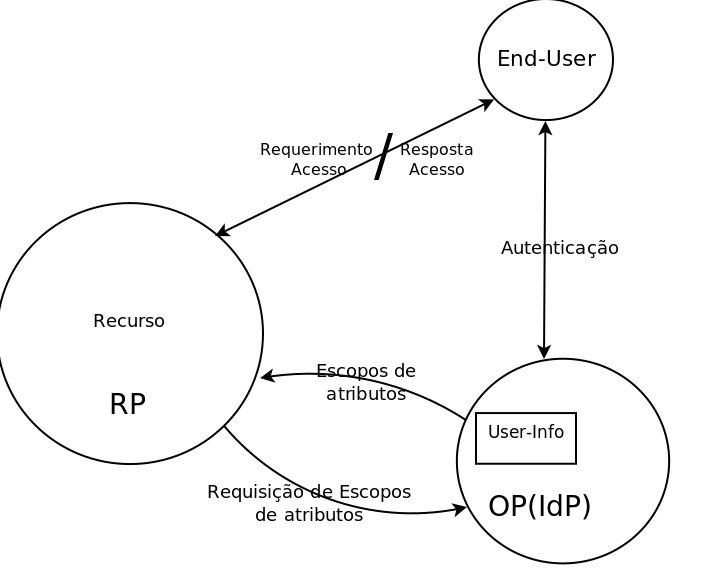
\includegraphics[height=5cm]{figuras/figura-proposta-especificacao-atual}
%		\label{Especificação atual do \textit{OpenID Connect}.}
%	}
%	\quad %espaco separador
%	\subfigure[Esquema geral da proposta]{
%		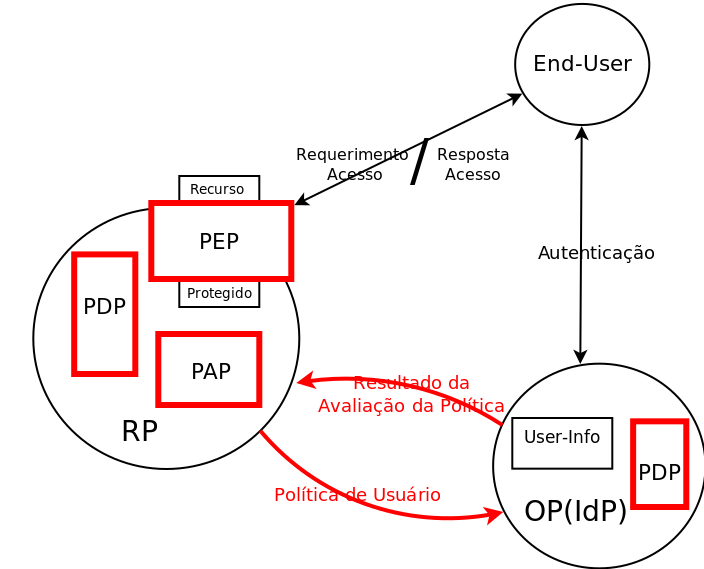
\includegraphics[height=5cm]{figuras/figura-proposta-modelo-proposto}
%		\label{Esquema geral da proposta do modelo.}
%	}
%	\caption{Esquemas demonstrando a especificação atual (à esquerda) e as modificações para acomodar a proposta do modelo.}
%	\label{fig-proposta-geral-colorido-subfiguras}
%\end{figure}


\section{Resultados esperados}\label{sec:result_esperados}

Para validar o modelo de autorização, mantendo a privacidade, será estabelecido um caso de uso, no qual serão criadas políticas de controle de acesso que atendam a maior parte dos requisitos. Como a avaliação de políticas pelos pontos de avaliação (PDP) já estão bem definidos, espera-se que a proposta possa ser validada sem problemas.

Em termos de desempenho, não há um trabalho relacionado que possa servir de parâmetro para quantificar o custo relativo da proposta. Mas, considerando que há necessidade de estender dois protocolos e incluir mais código de transporte, comunicação e avaliação de política, o desempenho tende a diminuir, aumentando a latência das decisões. Há duas questões que surgem para diminuir o impacto: a primeira seria a otimização, tanto dos códigos quanto das transações, isso após validar quanto à correção; a segunda, é considerar que essa proposta se destina a operações de controle de acesso que demandam intervenção humana na questão do consentimento, o que pode minorar a expectativa de latência nas respostas. O maior impacto poderia ocorrer no provedor de serviço, que poderia adotar soluções como otimização de avaliação de políticas de XACML \cite{mourad2014towards} e distribuição dos processos num ambiente paralelo.



\section{Validation of model}



\section{Conclusions}


This paper presents a new approach to realize fine-grained access control in environment with a identity provider OpenID Connect supplying PII data. The user controls the releasing the personal information. By adopting the evaluation of the service policies in the same domain of the identity provider, the personal data do not needs to be transported to the service provider. As a result of this, the privacy of PII is obtained and the user do not need care of the potential use of personal data by service providers. Important characteristic of this schema is the usability, because the user not need to established privacy policies concerning of manipulating his data.
Future works go in direction of research the monitoring and auditing of privacy protection provided by the IdP and on the other side there is the question of decomposition of policy and include this in the model presents in this paper.


\section*{Acknowledgements}
The authors would like to acknowledge the support from the LRG-UFSC.

\bibliographystyle{apsr}
\bibliography{bibliografia}


\end{document}
